\subsection{FactorGraph}

The FactorGraph class represents a single factor graph and contains a collection of all factors and variables associated with that factor graph.

\subsubsection{Constructor}

\ifmatlab
\begin{lstlisting}
FactorGraph([boundaryVariables])
\end{lstlisting}
\fi

\ifjava
\begin{lstlisting}
FactorGraph(VariableBase ... boundaryVariables)
\end{lstlisting}
\fi

For a basic factor graph, the constructor is simply the command FactorGraph with no arguments.

For a nested factor graph (one that may be used as a sub-graph within another graph), the constructor must include a list of the boundary variables of the graph.  When used as a sub-graph, the boundary variables are dummy variables with the same specification as the variables in the outer graph that will ultimately connect to the sub-graph.  A graph defined with boundary variables may alternatively be used as a top-level graph, in which case the boundary variables are used directly.

\subsubsection{Properties}

\para{Solver}
\label{sec:FactorGraph.Solver}

Read-write.  Indicates the choice of solver to be used for performing inference on the graph.  The default solver is SumProduct.

When setting the solver, the solver is given by a string representing the name of the solver.  The solver name is case insensitive.

\ifmatlab
\begin{lstlisting}
fg.Solver = 'SolverName';
\end{lstlisting}

The current set of valid solver names are:

\begin{itemize}
\item SumProduct
\item MinSum
\item Gaussian
\item ParticleBP
\item Gibbs
\item LP
\end{itemize}

\fi

\ifjava
\begin{lstlisting}
fg.setSolver(new com.analog.lyric.dimple.solvers.sumproduct.Solver());
\end{lstlisting}

The current set of valid solvers are:

\begin{itemize}
\item com.analog.lyric.dimple.solvers.sumproduct.Solver
\item com.analog.lyric.dimple.solvers.minsum.Solver
\item com.analog.lyric.dimple.solvers.gaussian.Solver
\item com.analog.lyric.dimple.solvers.particleBP.Solver
\item com.analog.lyric.dimple.solvers.gibbs.Solver
\item LP - The Java LP solver is not currently supported.
\end{itemize}

\fi


A description of each of these solvers is given in section~\ref{sec:SolversAPI}.

Note that the solver can be modified at any time.  After running the solver on a graph, the solver may be modified and the new solver run using the same graph\footnote{In this case, care must be taken to set any solver-specific parameters to the new values after changing the solver.}.  One exception is that if solver-specific built-in factors (also referred to as ``custom factors'') are used in a graph, it is not possible to switch solvers (a list of solver-specific built-in factors is given in section~\ref{sec:solverSpecificBuiltInFactors}).


\para{Scheduler}
\label{sec:FactorGraph.Scheduler}

Read-write.  Indicates the scheduler to be used for performing inference on the graph (unless a custom schedule is specified instead).  A scheduler defines a rule that determines the update schedule of a factor graph when performing inference.

When setting the scheduler, the scheduler is given by a string representing the name of the scheduler.  The scheduler name is case \emph{sensitive}.

\ifmatlab
\begin{lstlisting}
fg.Scheduler = 'SchedulerName';
\end{lstlisting}
\fi

\ifjava
\begin{lstlisting}
fg.setScheduler(new com.analog.lyric.dimple.schedulers.TreeOrSequentialScheduler());
\end{lstlisting}
\fi

Each scheduler is applicable only to a certain subset of solvers.  The list of all available built-in schedulers and a description of their behavior can be found in section~\ref{sec:Schedulers}.

\para{Schedule}
\label{sec:FactorGraph.Schedule}

\ifmatlab
Read-write.  Specifies a custom schedule to be used for performing inference.  A custom schedule is in the form of a list of nodes or edges in the graph to be updated.  Specifically, a cell array where each entry is either a node in the graph (either variable or factor), or a cell array containing a neighboring pair of nodes (\{variable, factor\} or \{factor, variable\}).  The order of the entries in the cell array indicate the order that updates should be performed in a single iteration (or scan) when performing inference.  Examples of using custom schedules are given in section~\ref{sec:CustomSchedules}.
\fi

\ifjava
Read-write.  Specifies a custom schedule to be used for performing inference.  Schedules must implement the ISchedule interface which provides an iterator over schedule entries.  Users can instantiate a FixedSchedule object and add nodes and/or edges to the fixed schedule to provide an order of updates.  Examples of using custom schedules are given in section~\ref{sec:CustomSchedules}.
\fi

For all BP solvers, any of these entries may be included, and have the following interpretation.

\ifmatlab
\begin{description}
\item[Variable] Update messages for all outgoing edges of that variable.
\item[Factor] Update messages for all outgoing edges of that factor.
\item[\{Variable, Factor\}] Update a single outgoing edge of the variable in the direction connecting to the specified factor.
\item[\{Factor, Variable\}] Update a single outgoing edge of the factor in the direction connecting to the specified variable.
\end{description}
\fi

\ifjava
\begin{description}
\item[FixedSchedule.add(variable)] Update messages for all outgoing edges of that variable.
\item[FixedSchedule.add(factor)] Update messages for all outgoing edges of that factor.
\item[FixedSchedule.add(variable,factor)] Update a single outgoing edge of the variable in the direction connecting to the specified factor.
\item[FixedSchedule.add(factor,variable)] Update a single outgoing edge of the factor in the direction connecting to the specified variable.
\end{description}
\fi

For BP solvers, a check is made when a custom schedule is set to ensure that all edges in the graph are updated at least once.

For the Gibbs solvers, the Schedule should include only variable entries.  Any other entries will be ignored.

If a custom schedule is set on a factor graph (either an entire graph or a sub-graph), this schedule is used instead of any built-in scheduler that may have previously been set (or the default scheduler).

In a nested graph, the Schedule property at each nesting level may be set independently.  For some built-in schedulers, the user may mix custom schedules at some nesting layers, while using built-in schedulers at others.  The particular built-in schedulers that support such mixing are described in section~\ref{sec:FactorGraph.Scheduler}.


\para{NumIterations}

Read-write.  The NumIterations property sets the number of iterations BP will to run when using the solve method.  This only applies to solvers that use BP, which are the SumProduct, MinSum, Gaussian, and ParticleBP solvers.

The default value is 1.  For a factor graph with a tree-structure, when using the default scheduler, one iteration is appropriate.  Otherwise, it would normally be appropriate to set the number of iterations to a larger value.

\para{NumSteps}

Read-write.  This property is used for rolled-up graphs (see section~\ref{sec:rolledUpFactorGraphs}).  This property determines the number of steps over which to perform inference when using the solve or continueSolve methods (see sections~\ref{sec:FactorGraph.solve} and~\ref{sec:FactorGraph.continueSolve}).  A \emph{step} corresponds to a single run of the solver over the current portion of the rolled-up graph, followed by advancing the graph to the next position.  By default, this property is infinite, resulting in no limit to the number of steps to be run (running until there is no more source data).

\para{Name}

Read-write.  When read, retrieves the current name of the factor graph.  When set, modifies the name of the factor graph to the corresponding value.  The value set must be a string.

\ifmatlab
\begin{lstlisting}
fg.Name = 'string';
\end{lstlisting}
\fi

\ifjava
\begin{lstlisting}
fg.setName('string');
\end{lstlisting}
\fi

\para{Label}

Read-write.  All variables and factors in a Factor Graph must have unique names.  However, sometimes it is desirable to have variables or factors share similar strings when being plotted or printed.  Users can set the Label property to set the name for display.  If the Label is not set, the Name will be used for display.  Once the label is set, the label will be used for display.


\para{Score}
\label{sec:FactorGraph.Score}

Read-only.  When read, computes and returns the score (energy) of the graph given a specified value for each of the variables in the graph.  The score represents the energy of the graph given the specified variable configuration, including all factors as well as all Inputs to variables (which behave as single-edge factors).  The score value is relative, and may be arbitrarily normalized by an additive constant.  The value of the score corresponds to the sum over factors and variables of their corresponding scores (see sections~\ref{sec:Factor.Score} and~\ref{sec:Variable.Score}).

The value of each variable used when computing the Score is the Guess value for that variable (see section~\ref{sec:Variable.Guess}).  If no Guess had yet been specified for a given variable, the value with the most likely belief (which corresponds to the Value property of the variable) is used\footnote{For some solvers, beliefs are not supported for all variable types; in such cases there is no default value, so a Guess must be specified.}.

For a rolled-up graph, the Score property represents only the score for only the portion of the graph in the current buffer.


\para{BetheFreeEnergy}
\label{sec:FactorGraph.BetheFreeEnergy}

Read-only.  (Only applies to the Sum Product Solver).  When read returns:

\[
BetheFreeEnergy = InternalEnergy - BetheEntropy
\]

\ifjava
\begin{lstlisting}
double bfe = fg.getBetheFreeEnergy();
\end{lstlisting}
\fi

\para{Internal Energy}
\label{sec:FactorGraph.InternalEnergy}

Read-only.  (Only applies to the Sum Product Solver).  When read returns:

\[
InternalEnergy = \sum_{a \in F }InternalEnergy(a) + \sum_{i \in V}InternalEnergy(i)
\]

Where F is the set of all Factors and V is the set of all variables.  If Dimple treated inputs as single node Factors, this method would only sum over factors.

For a definition of a Factor's InternalEnergy, see sections~\ref{sec:Factor.InternalEnergy}.  For a definition of a Variable's InternalEnergy, see section~\ref{sec:Variable.InternalEnergy}.

\ifjava
\begin{lstlisting}
double ie = fg.getInternalEnergy();
\end{lstlisting}
\fi

\para{Bethe Entropy}
\label{sec:FactorGraph.BetheEntropy}

Read-only.  (Only applies to the Sum Product Solver).  When read returns:

\[
 BetheEntropy = \sum_{a \in F}BetheEntropy(a) - \sum_{i \in V}(d_i-1) BetheEntropy(i) 
 \]

Where F is the set of all Factors, V is the set of all variables, and $d_i$ is the degree of variable $i$ (i.e. the number of factors $i$ is connected to).

For a definition of a Factor's BetheEntropy, see sections~\ref{sec:Factor.BetheEntropy}.  For a definition of a Variable's InternalEnergy, see section~\ref{sec:Variable.BetheEntropy}.

\ifjava
\begin{lstlisting}
be = fg.getBetheEntropy();
\end{lstlisting}
\fi


\subsubsection{Methods}

\para{addFactor}
\label{sec:FactorGraph.addFactor}

\begin{lstlisting}
MyGraph.addFactor(factorSpecification, variableList);
\end{lstlisting}

The addFactor method is used to add a factor to a factor-graph, connecting that factor to a specified set of variables. There are several ways of specifying the factor.  The method takes a factorSpecification argument followed by a comma-separated list of variables or variable arrays.

The list of variables or variable arrays indicate which variables to connect to the factor.  The order of the variables listed must correspond to the order of edges of the factor.   \ifmatlab  In the case of variable arrays, the array is flattened to a one-dimensional form using the usual MATLAB ordering, defining the order of the individual variables in the array.  In this ordering, the array is scanned in successive dimensions, beginning with the first (row) dimension (equivalent to the MATLAB \texttt{(:)} operator). \fi

Some of the variables may be replaced by constants.  In this case, no variable is created, but instead the specified constant value is used in place of a variable for the corresponding edge of the factor.  The value of a constant must be a valid value given the definition of the corresponding factor.  \ifmatlab Constants may be arrays, but in this case, they are not flattened.  Instead they are treated as array-valued constants\footnote{This is because Dimple supports variables that have domains for which individual domain elements are arrays.}.  \fi

The factorSpecification may be specified in one of a number of different ways.  The following table lists the various ways the factorSpecification can be specified:

\ifmatlab
\begin{longtable} {l p{10cm}}
Factor Specification & Description \\
\hline
\endhead
%
functionHandle & The MATLAB function handle for a factor function.  A factor function written in MATLAB is a function that takes arguments corresponding values from the domain of each of the connected variables (in the order listed) and returns a non-negative weight corresponding to the unnormalized value of the factor.  In MATLAB, the function handle of a function is indicated using the \texttt{@} operator, for example, \texttt{@myFactor}.  Anonymous functions are also supported.  Specifying a factor in this form is supported only if all connected variables are discrete.  \\
%
FactorTable & A FactorTable object as described in section~\ref{sec:FactorTable}.  Specifying a factor in this form is supported only if all connected variables are discrete. \\
%
indexList, weightList & A factor table specified in an alternative form.  The indexList and weightList arguments are defined identically to their definition in the FactorTable constructor described in section~\ref{sec:FactorTable}. Specifying a factor in this form is supported only if all connected variables are discrete. \\
%
weightArray & A factor table specified in an alternative form.  The weightArray argument is defined identically to its definition in the FactorTable constructor described in section~\ref{sec:FactorTable}. Specifying a factor in this form is supported only if all connected variables are discrete. \\
%
builtInFactorName & String indicating the name of a built-in factor.  The list of Dimple built-in factors is given in section~\ref{sec:builtInFactors}.  Built-in factor names are case sensitive.  \\
%
FactorFunction & A FactorFunction object as described in section~\ref{sec:FactorFunction}. This form can be used to specify a built-in factor that requires constructor arguments.  The list of Dimple built-in factors is given in section~\ref{sec:builtInFactors}.\\
%
factorFunctionAltForm & A factor function specified in an alternative form.  The form is a cell array, where the first entry is a string indicating the name of the built-in factor, and the remaining entries are constructor arguments for the built-in factor.  \\
%
FactorGraph & A sub-graph to be nested within this graph.  The number and order of the variables listed in the variableList must correspond to the number and order of the boundary variables declared when the sub-graph was created.  When adding a nested graph within an outer graph, the specified sub-graph is used as a template to create a new factor graph that is actually added to the outer graph.  Copies are made of all of the variables and factors in the specified sub-graph. \\
%
javaFactorFunction & The fully-qualified name of a Java FactorFunction class.  Creation of custom Java FactorFunctions is described in Appendix~\ref{sec:userJava}. \\
\end{longtable} 
\fi

\ifjava
\begin{longtable} {l p{10cm}}
Factor Specification & Description \\
\hline
\endhead
%
FactorFunction & A FactorFunction object as described in section~\ref{sec:FactorFunction}. This form can be used to specify a built-in factor that requires constructor arguments.  The list of Dimple built-in factors is given in section~\ref{sec:builtInFactors}.\\
%
FactorTable & A FactorTable object as described in section~\ref{sec:FactorTable}.  Specifying a factor in this form is supported only if all connected variables are discrete. \\
%
FactorGraph & A sub-graph to be nested within this graph.  The number and order of the variables listed in the variableList must correspond to the number and order of the boundary variables declared when the sub-graph was created.  When adding a nested graph within an outer graph, the specified sub-graph is used as a template to create a new factor graph that is actually added to the outer graph.  Copies are made of all of the variables and factors in the specified sub-graph. \\
\end{longtable} 

\fi


\ifmatlab
\para{addFactorVectorized}
\label{sec:FactorGraph.addFactorVectorized}

To get reasonable speed out of MATLAB, one needs to vectorize their code.  If a user wishes to build a FactorGraph with large numbers of factors in a regular arrangement, they will want to avoid making many calls to addFactor.  The addFactorVectorized method can be used instead to create many factors at once.

\begin{lstlisting}
fg.addFactorVectorized(factorSpecification, variableList);
\end{lstlisting}

Using addFactorVectorized is very similar to using addFactor.  The factorSpecification is defined identically to addFactor (see section~\ref{sec:FactorGraph.addFactor}). The variableList is similar, but includes some options for customizing how vectorization is done.

In the simplest case, the variableList includes a comma-separated list of variable arrays, all with the same dimensions.  In this case, the result is creation of an array of factors with the same dimensions as the variables, where one element of each of the listed variable arrays is connected to the corresponding factor in the factor array.

One or more of the variables in the variableList may be a scalar (single variable) rather than an array.  In this case, that variable is connected to all of the factors in the created factor array.  The other variables in the variableList that are not scalars must all have the same dimensions.

In some cases, it may be useful to vectorize over some dimensions of a variable, but have other dimensions be flattened and connect to each individual factor in the factor array.  In such cases, an entry in the variable list may be specified as a cell array containing two elements:

\begin{itemize}
\item The variable array
\item A vector of indices, where each index represents a dimension over which the variable should be vectorized.
\end{itemize}

For example:
\begin{lstlisting}
A = Bit(100,100);
B = Bit(100,100,5);
fg.addFactorVectorized(factorSpecification, A, {B, [1 2]});
\end{lstlisting}

For variable B, first two dimensions, of size 100x100 correspond to the 100x100 factors that we wish to vectorize factor creation.  Since dimension 3 was not included in this list, then for each value of row and column dimension, the entire length of B variables in the third dimension are connected to the corresponding factor.

The vectorized dimensions for all non-scalar variables must be of the same size.

As in addFactor, some of the variables in variableList may be replaced with constants.  In this case, every copy of the factor in the factor array uses the same constant value.

Further description and examples of using addFactorVectorized is given in section~\ref{sec:vectorizedFactorCreation}.
\fi

\ifmatlab
\para{addFactorNoCache}
\label{sec:addFactorNoCache}

When creating a factor for discrete variables, Dimple attempts to determine if the resulting factor tables would be the same as any previously created factors.  If so, it shares the factor table to save space.  In some cases, it may not be desirable for certain factors to share a factor table (for example if entries in one of the factor tables will later be modified).  In such cases, the addFactorNoCache method can be used in lieu of the addFactor method.  The interface for the addFactorNoCache is identical to that of the addFactor method.

\fi

\ifmatlab
\para{addDirectedFactor}

When adding a factor that will be designated as directed, this method provides a shorthand way to indicate this on factor creation.

\begin{lstlisting}
fg.addDirectedFactor(factorSpecification, variableList, directedTo);
\end{lstlisting}

The factorSpecification is defined identically to addFactor (see section~\ref{sec:FactorGraph.addFactor}).

Instead of being a comma-separated list, the variableList argument is a cell array containing the list of variables or variable arrays to be connected to the factor.  Otherwise, the behavior of the variable list is the same as for the addFactorMethod.

The directedTo argument is a cell array containing a subset of the variables listed in the variableList, specifically, the set of variables that are directed outputs of the factor.

Using addDirectedFactor is equivalent to the following (where the variableList in this case is a comma-separated list instead of a cell array):

 \begin{lstlisting}
f = fg.addFactor(factorSpecification, variableList);
f.directedTo(directedTo);
\end{lstlisting}

\fi

\para{initialize}

\begin{lstlisting}
MyGraph.initialize();
\end{lstlisting}

The initialize method resets the state of the factor graph and its associated solver.  When performing inference incrementally, for example using the iterate method, the initialize method must be called before the first iterate call.  When using the solve method to perform inference, there is no need to call initialize first.  The initialize method takes no arguments.

\para{solve}
\label{sec:FactorGraph.solve}

\begin{lstlisting}
MyGraph.solve();
\end{lstlisting}

The solve method runs the solver on the factor graph for the specified duration.  Calling solve initializes the graph prior to solving.

For BP-based solvers, the solver runs the number of iterations specified by the NumIterations property.  For the Gibbs solver, it runs for the specified number of samples (see section~\ref{sec:GibbsSolverAPI}).

For rolled-up factor graphs, the solver runs the solver over multiple steps of the graph.  A \emph{step} corresponds to a single run of the solver over the current portion of the rolled-up graph, followed by advancing the graph to the next position.  It performs the number of steps of inference specified by the NumSteps property or until there is no more data in a data source, whichever comes first.


\para{continueSolve}
\label{sec:FactorGraph.continueSolve}

This method is used for manually advancing a rolled-up graph (see section~\ref{sec:manuallyAdvancingRolledUpGraph}).  This method takes no arguments and returns no value.  When called, it performs the number of steps of inference specified by the NumSteps property or until there is no more data in a data source, whichever comes first.  A \emph{step} corresponds to a single run of the solver over the current portion of the rolled-up graph, followed by advancing the graph to the next position.  The initialize method should be called prior to calling this method for the first time on an entire rolled-up graph, but should not be called before calling this method again to run additional steps.

\para{solveOneStep}

This method is used for manually advancing a rolled-up graph (see section~\ref{sec:manuallyAdvancingRolledUpGraph}).  This method takes no arguments and returns no value.  When called, it performs inference on the current portion of the rolled-up graph.  Inference is performed on this section of the graph using whatever solver-specific parameters had previously been specified.  The graph is not re-initialized prior to performing inference, starting instead from the final state resulting from inference on the previous graph position.  The initialize method should be called prior to calling this method for the first time on an entire rolled-up graph, but should not be called after each advance to the next section.

\para{advance}

This method is used for manually advancing a rolled-up graph (see section~\ref{sec:manuallyAdvancingRolledUpGraph}).  This method takes no arguments and returns no value.  When called, it advances the graph to the next position.  Advancing the graph involves getting the next value of all data sources, and writing the next available value to all data sinks.

\para{hasNext}

This method is used for manually advancing a rolled-up graph (see section~\ref{sec:manuallyAdvancingRolledUpGraph}).  This method takes no arguments.  It returns a boolean value indicating whether or not it is possible to advance the graph to the next position.  This will be true only if all of the data sources have at least one more available value.

\para{baumWelch}
\label{sec:FactorGraph.BaumWelch}

\begin{lstlisting}
fg.baumWelch(factorList, numRestarts, numSteps);
\end{lstlisting}

The baumWelch method performs the Expectation-Maximization (EM) algorithm on a factor graph (the specific case of EM on an HMM graph is called the Baum-Welch algorithm, though EM in Dimple can be applied to any graph structure).

This method has the following limitations:

\begin{itemize}
\item The factors on which parameter estimation is being performed must be directed (see section~\ref{sec:Factor.DirectedTo}).
\item The factors on which parameter estimation is being performed must be connected only to discrete variables.
\item The factors on which parameter estimation is being performed must \emph{not} be solver-specific built-in factors (also known as custom factors, see section~\ref{sec:solverSpecificBuiltInFactors}).
\item The Solver must be set to use the SumProduct solver (the default solver).
\end{itemize}

The factorList argument is either a single Factor or FactorTable, or a cell array of Factors or FactorTables.  The weight values in these factor tables are the parameters to be estimated.  All other factors in the graph remain fixed and unmodified.  When including a FactorTable, if that table is used in more than one factor in the graph, the entries in the table are tied, estimating them jointly for all factors containing that table.

The numRestarts argument indicates the number of times the EM process is repeated using distinct random restart values for the parameters.  When numRestarts is greater than 1, the EM process is repeated with different random initialization, and the final resulting parameter values are chosen from the run that resulted in the smallest Bethe free energy for the graph.

The numSteps argument indicates (for each restart), how many steps of the EM algorithm are to be run.  A single step of the EM algorithm is one run of belief propagation followed by re-estimation of the parameter values.

Note that the number of iterations for each run of belief propagation is determined from the NumIterations property.  If the graph is a tree, the number of iterations should be 1 (the default value).  If the graph is loopy, it should be set to a larger value (in this case, the EM algorithm is only approximate).

Upon completion of this method, the result appears in the factor tables that were listed in the factorList argument.  That is, the factor table weights contain the resulting estimated values.  To read these values, the Weights property of the factor table can be read (see section~\ref{sec:FactorTable}).  For a factor, the factor table can be extracted using the FactorTable property (see section~\ref{sec:FactorTable}), and then the weights can be read from that.


\para{join}

The join method can be used to join a set of existing variables or a set of existing factors in a graph.  In the current version of Dimple this method is supported only for discrete variables, and factors connected only to discrete variables.

When joining variables, the join method is called with a comma-separated list of variables to be joined.

\begin{lstlisting}
fg.join(variableList);
\end{lstlisting}

The result is a new variable with a domain that is the Cartesian product of the domains of all of the variables being joined.

When joining factors, the join method is called with a comma-separated list of factors to be joined.

\begin{lstlisting}
fg.join(factorList);
\end{lstlisting}

The result is a new factor with a factor table that corresponds to the product of the factors being joined.  The new factor connects with the union of all variables that were previously connected to any of the joined variables.


\para{split}

The split method splits a variable in an existing graph into two variables connected by an Equality factor.

\begin{lstlisting}
fg.split(variable, [factorList]);
\end{lstlisting}

The method takes an optional comma-separated list of factors.  This list of factors identifies factors already connected to the variable that are to be moved to the new instance of the variable.  All unspecified factors remain connected to the original instance.

\para{removeFactor}

\begin{lstlisting}
fg.removeFactor(factor);
\end{lstlisting}

This method removes the specified factor from an existing factor graph that contains it.  This also removes all edges that connect this factor to neighboring variables.

\ifmatlab
\para{plot}

The plot method is used to visualize a factor graph or a portion of a factor graph.  Examples of various use cases for plotting factor graphs are given in section~\ref{sec:PlottingAGraph}.

The plot method may be called with no arguments, or with a set of optional arguments.  The optional arguments are defined in the following table.  These are in the form of names (as strings) followed by one or more values.

\begin{longtable} {l p{3cm} p{10cm}}
Name & Values & Description \\
\hline
\endhead
\texttt{'labels'} & true/false & Boolean value indicating whether or not to display the name of each variable and factor node.  By default labels are not displayed. \\
\texttt{'color'} & [nodeList], color & Specifies the color of some or all nodes in the graph.  If no nodeList is included, then this specifies the color of all nodes in the graph.  If nodeList is specified, then the color applies to only the listed nodes.  The nodeList argument is a cell-array of nodes in the graph (factors and variables).  The color argument is a string indicating a MATLAB color (e.g., 'r').  More than one set of 'color' arguments may appear in a single call to plot. \\ 
\texttt{'nodes'} & nodeList & Indicates the set of nodes in the graph to be included in the plot.  The nodeList argument is a cell-array of nodes in the graph (factors and variables).  By default the entire graph is plotted.  \\
\texttt{'depth'} & rootNode, depth & This argument indicates a portion of the graph to be displayed by specifying a root node and depth (distance) from that node.  The plot includes only the root node and all other nodes that are within the specified distance from the root.  By default the entire graph is plotted.  \\
\texttt{'nesting'} & nestingDepth & By default, the plotting method ignores hierarchy and plots the flattened graph.  The nesting argument specifies how deep to descend into the nesting hierarchy before considering nested graphs to be factors and plotting them as such. \\
\end{longtable}

\fi

\para{addBoundaryVariables}
\begin{lstlisting}
fg.addBoundaryVariables([factorList]);
\end{lstlisting}

This method takes a comma separated list of variables. The listed variables can then be used as boundary variables in a nested graph.

\ifmatlab
\begin{lstlisting}

ng = FactorGraph();
a = Bit(2,1);
y = a(1) + a(2);
ng.addBoundaryVariables(y,a);

fg = FactorGraph(); 
y = Discrete(0:2);
a = Bit(2,1);
fg.addFactor(ng,y,a);
a.Input = [1 0];
fg.solve();

\end{lstlisting}
\fi

\ifjava
\begin{lstlisting}
FactorGraph ng = new FactorGraph();
Bit a = new Bit();
Bit b = new Bit();
		
Equals eq = new Equals();
		
ng.addFactor(eq,a,b);
		
ng.addBoundaryVariables(a,b);
		
FactorGraph fg = new FactorGraph();
Bit a2 = new Bit();
Bit b2 = new Bit();
fg.addFactor(ng,a2,b2);
\end{lstlisting}
\fi

\subsubsection{Introspection}

The FactorGraph class provides several feature for inspecting aspects of the graph.  The ability to nest graphs complicates things a bit.  Nested FactorGraphs can be considered Factors.  All of the introspection features allow the user to view nested graphs as leaf factors or to descend into them and operate on the children of the nested graphs.  Each feature provides several methods:

\begin{itemize}
\item $<$FeatureName$>$(int relativeNestingDepth) -- The relativeNestingDepth specifies how deep to descend into the nested FactorGraphs before treating deeper NestedGraphs as Factors.  Specifying 0 will treat the top level nested Graphs as factors.  Specifying a large enough number will descend all the way to the leaf factors.  Specifying something between 0 and the FactorGraph's maximum depth will descend as far as this parameter specifies before considering NestedGraphs to be factors.  The parameter contains the word ``relative'' because users can retrieve nested graphs.  They can call one of the feature's methods on that nested graph.  
\item $<$FeatureName$>$Flat() -- equivalent of $<$FeatureName$>$(max int)
\item $<$FeatureName$>$Top() -- equivalent of $<$FeatureName$>$(0)
\item $<$FeatureName$>$() -- equivalent of $<$FeatureName$>$Flat().  It was thought that users will most often want to operate on the FactorGraph in its flattened form.
\end{itemize}

Now, on to the specific features.

\para{Retrieving All Factors}

Users can retrieve Factors and/or NestedGraphs associated with a graph using the Factors methods and properties:

\ifmatlab
\begin{itemize}
\item Fg.Factors
\item Fg.FactorsFlat
\item Fg.FactorsTop
\item Fg.getFactors(relativeNestingDepth)
\end{itemize}
\fi

\ifjava
\begin{itemize}
\item Fg.getFactors()
\item Fg.getFactorsFlat()
\item Fg.getFactorsTop()
\item Fg.getFactors(relativeNestingDepth)
\end{itemize}
\fi

When the user specifies a relativeNestingDepth or calls FactorsTop, the resulting cell array will contain a mix of leaf factors and Nested Graphs.

\para{Retrieving Factors but Not Nested Factor Graphs}

The FactorGraph class provides the following:

\ifmatlab
\begin{itemize}
\item NonFactorGraphFactors
\item NonFactorGraphFactorsFlat
\item NonFactorGraphFactorsTop
\item getNonFactorGraphFactors(relativeNestingDepth)
\end{itemize}
\fi

\ifjava
\begin{itemize}
\item getNonFactorGraphFactors()
\item getNonFactorGraphFactorsFlat()
\item getNonFactorGraphFactorsTop()
\item getNonFactorGraphFactors(relativeNestingDepth)
\end{itemize}
\fi


As the name implies, this will behave similar to the Factors properties and methods but will exclude nested graphs.

\para{Retrieving Variables}

The FactorGraph class provides the following:

\ifmatlab
\begin{itemize}
\item Variables -- calls VariablesFlat
\item VariablesFlat -- Returns a list of all the Variables in the graph, including those contained by nested graphs.
\item VariablesTop -- Returns only those variables contained in the top level of the graph.
\item getVariables(relativeNestingDepth,forceIncludeBoundaryVariables) -- Returns all variables contained in the FactorGraph from which the method is called as Variables that are as deep as the specified relativeNestingDepth.  The second parameter is optional and defaults to false.  When false, boundary variables are only included by the root graph.  When true, boundary variables are included regardless of whether a graph is a root or nested graph.
\end{itemize}
\fi

\ifjava
\begin{itemize}
\item getVariables() -- calls getVariablesFlat()
\item getVariablesFlat() -- Returns a list of all the Variables in the graph, including those contained by nested graphs.
\item getVariablesTop() -- Returns only those variables contained in the top level of the graph.
\item getVariables(relativeNestingDepth,forceIncludeBoundaryVariables) -- Returns all variables contained in the FactorGraph from which the method is called as Variables that are as deep as the specified relativeNestingDepth.  The second parameter is optional and defaults to false.  When false, boundary variables are only included by the root graph.  When true, boundary variables are included regardless of whether a graph is a root or nested graph.
\end{itemize}
\fi


\para{Retrieving All Nodes}

The FactorGraph provides the following:

\ifmatlab
\begin{itemize}
\item Nodes
\item NodesFlat
\item NodesTop
\item getNodes(relativeNestingDepth,forceIncludeBoundaryVariables)
\end{itemize}
\fi

\ifjava
\begin{itemize}
\item getNodes()
\item getNodesFlat()
\item getNodesTop()
\item getNodes(relativeNestingDepth,forceIncludeBoundaryVariables)
\end{itemize}
\fi

These methods call the Factor and Variable methods and concatenate the results together.

\para{Determining if a FactorGraph is a tree}

The FactorGraph class provides the following:

\ifmatlab
\begin{itemize}
\item isTree(relativeNestingDepth) 
\item isTreeTop 
\item isTreeFlat 
\end{itemize}
\fi

\ifjava
\begin{itemize}
\item isTree(relativeNestingDepth) 
\item isTreeTop()
\item isTreeFlat()
\end{itemize}
\fi


isTree -- Users can call <factor graph name>.isTree() to determine if a FactorGraph is a tree.  If the graph contains cycles, this method will return false. Like the other methods, the relativeNestingDepth determines at what point to consider NestedGraphs to be leaf cells.  

\para{Retrieving an Adjacency Matrix}

All of the following methods return a pair: [A, labels] where A is a square connectivity matrix and labels is a cell array of strings specifying the names of the nodes in A. 

\begin{itemize}
\item getAdjacencyMatrix(relativeNestingDepth,forceIncludeBoundaryVariables) -- relativeNestingDepth behaves the same as in other methods that take this parameter.  So does forceIncludeBoundaryVariables. forceIncludeBoundaryVariables has a default value of false.
\item getAdjacencyMatrix(nodes,forceIncludeBoundaryVariables) -- Users can specify a specific subset of nodes in which they are interested.  This method will return an adjacency matrix with only those nodes.  Nodes are considered connected only if there is an edge directly connecting them.
\item getAdjacencyMatrixTop() -- equivalent to getAdjacencyMatrix(0,false)
\item getAdjacencyMatrixFlat() -- equivalent to getAdjacencyMatrix(intmax,false)
\end{itemize}

FactorGraph also provides an AdjacencyMatrix Property:

\begin{itemize}
\item AdjacencyMatrix -- equivalent to getAdjacencyMatrixFlat and only returns A (not the labels).  \ifmatlab MATLAB properties can only return one object. \fi
\end{itemize}

An example of getAdjacencyMatrix:

\ifmatlab
\begin{lstlisting}
fg = FactorGraph();
b = Bit(2,1);
b(1).Name = 'b1';
b(2).Name = 'b2';
f = fg.addFactor(@xorDelta,b);
f.Name = 'f';
[A,labels] = fg.getAdjacencyMatrix();
A =

     0     0     1
     0     0     1
     1     1     0


labels = 

    'b1'
    'b2'
    'f'
\end{lstlisting}
\fi

\ifjava
\begin{lstlisting}
FactorGraph fg = new FactorGraph();
Bit b1 = new Bit();
b1.setName("b1");
Bit b2 = new Bit();
b2.setName("b2");
Equals ne = new Equals();
Factor f = fg.addFactor(ne,b1,b2);
f.setName("f");
MapList<INode> nodes = fg.getNodesFlat();
int [][] matrix = fg.getAdjacencyMatrix(nodes);
for (INode n : nodes)
	System.out.println(n);
for (int i = 0; i < matrix.length; i++)
	System.out.println(Arrays.toString(matrix[i]));
\end{lstlisting}

results in:

\begin{lstlisting}
b1
b2
f
[0, 0, 1]
[0, 0, 1]
[1, 1, 0]
\end{lstlisting}
\fi

\para{Depth First Search}

\begin{itemize}
\item depthFirstSearch(node, searchDepth, relativeNestingDepth) -- 
\begin{itemize}
\item node -- Specifies the node from which to initiate the search
\item searchDepth -- specifies how far from ``node'' the search should go.
\item relativeNestingDepth -- determines how deep to go down the NestedGraphs before considering NestedGraphs to be leaf cells. 
\end{itemize}
\item depthFirstSearchFlat(node, searchDepth) -- equivalent of depthFirstSearch(node,searchDepth,maxint)
\item depthFirstSearchThop(node, searchDepth) -- equivalent of depthFirstSearch(node,searchDepth,0)
\end{itemize}

An example:

\ifmatlab
\begin{lstlisting}
fg = FactorGraph();
b = Bit(6,1);
for i = 1:6
b(i).Name = sprintf('b%d',i);
end
f1 = fg.addFactor(@xorDelta,b(1:4));
f1.Name = 'f1';
f2 = fg.addFactor(@xorDelta,b(4:6));
f2.Name = 'f2';
 
nodes = fg.depthFirstSearch(b(1),3);
\end{lstlisting}

calling fg.plot('color',b(1),'g','labels',true) reveals the following structure of this graph

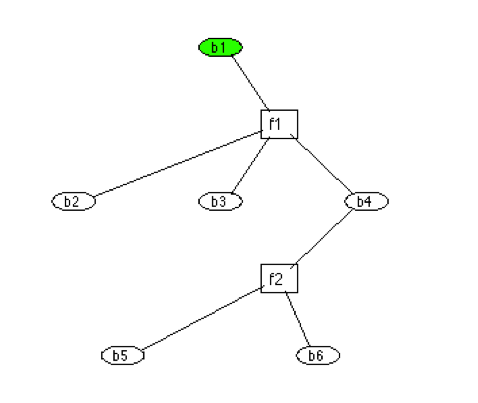
\includegraphics{images/Introspection.png}
 
As you might guess fg.depthFirstSearch(b(1),3) will return a collection of six nodes: b1, f1, b2, b3, b4, and f2.  It will not include b5 and b6 since those are at a depth of four from b1.
\fi

\ifjava
\begin{lstlisting}
FactorGraph fg = new FactorGraph();
Bit [] b = new Bit[6];
for (int i = 0; i < b.length; i++)
{
	b[i] = new Bit();
	b[i].setName("B" + i);
}
Factor f1 = fg.addFactor(new XorDelta(), b[0],b[1],b[2],b[3]);
f1.setName("f1");
Factor f2 = fg.addFactor(new XorDelta(), b[3],b[4],b[5]);
f2.setName("f2");
 
MapList<INode> nodes = fg.depthFirstSearch(b[0],3);

for (INode n : nodes)
{
	System.out.println(n);
}
\end{lstlisting}

results in:

\begin{lstlisting}
B0
f1
B1
B2
B3
f2
\end{lstlisting}
 
As you might guess fg.depthFirstSearch(b[0],3) will return a collection of six nodes: b0, f1, b1, b2, b3, and f2.  It will not include b5 and b6 since those are at a depth of four from b1.

\fi




